\documentclass[../../main.tex]{subfiles}

\graphicspath{{../../fig/}}
\setcounter{section}{0}

\begin{document}
\chapter{スパースワイヤーグリッドのたわみ量の評価}
\label{chap:wiresag_swg}
\ref{chap:wiresag}章にて、ワイヤーのたわみ量を自動で評価する装置を開発した。
本章では、開発した装置を用いて実際に偏光角較正に使用されるスパースワイヤーグリッドのたわみ量を評価する。
はじめに、評価するスパースワイヤーグリッドのワイヤーの張り方について述べ、次いで評価結果とその考察を行う。
その後、評価されたたわみ量が大きかったワイヤーを張り直すことで修繕を行い、再度評価を行った結果について述べる。
最後に今回のたわみ量の評価を通じて得られたスパースワイヤーグリッドのワイヤーの張り方に関する今後の展望について述べる。

\section{評価されたスパースワイヤーグリッドのワイヤーの張り方}
今回評価したスパースワイヤーグリッドは、\ref{subsec:wg_design}項で述べたように$\SI{230}{g}$の重りを使用し、
ワイヤー番号が奇数番目のものと偶数番目のものに分け、二回に分けてワイヤーを張ることで作成された。
このとき、はじめにワイヤー番号が奇数番目のものを張り、次にワイヤー番号が偶数番目のものを張った。

\section{評価結果とその考察}
図\ref{fig:wiresag_swg_result}(\subref{fig:wiresag_swg_sag_result})にスパースワイヤーグリッドのたわみ量の評価結果を示す。
横軸はワイヤー番号、縦軸はワイヤーのたわみ量を示している。
fitting errorを統計的な誤差として、前章にて得られた$\SI{15}{\micro m}$を系統的な誤差として、それらの2乗和の平方根をたわみ量の誤差として示した。
図中には測定されたたわみ量に加え、「理論値」として$\SI{230}{g}$の重りによって生まれるたわみ量(平均たわみ角にして$0.006\tcdegree$)を示した。
加えて、たわみ角が$0.02\tcdegree,\,0.05\tcdegree$(先行研究\cite{swg:murata}\cite{swg:iijima})に相当するたわみ量も参考のために示した。
図\ref{fig:wiresag_swg_result}(\subref{fig:wiresag_swg_sag_angle_result})には、
たわみ量をたわみ角に変換した結果を示す。横軸はワイヤー番号、縦軸はワイヤーのたわみ角を示している。
測定されたたわみ角の平均は$0.025\tcdegree$であるが、全体的に理論値よりもたわみが大きい。
その原因としては、ワイヤーをスパースワイヤーグリッドのアルミニウムリングに張る際にその端で急に曲げられるため、
実際にかかっている張力が重りの重さ\SI{230}{g}よりも小さくなっているためだと考えられる。

また、明らかにたわみ量が大きく、たわみ角が先行研究で評価された値$0.05\tcdegree$を超えるワイヤーが存在していた。
これらのワイヤーはすべて奇数番目のワイヤーであった。
図\ref{fig:wiresag_swg_even_odd}にワイヤー番号の偶奇によるたわみ角の違いを示す。
偶数番目のワイヤーのたわみ角を青点で示し、奇数番目のワイヤーのたわみ角を赤点で示している。
この図より、奇数番目のワイヤーのたわみ角が偶数番目のワイヤーに比べて大きい傾向にあることがわかる。
今回評価したスパースワイヤーグリッドは奇数番目のワイヤーから張り始めたことから、このたわみ角の違いは、
\begin{enumerate}
    \item 単に奇数番目のワイヤーを張るときにうまく張れなかった
    \item 後に張ったワイヤーによる張力によってスパースワイヤーグリッドのアルミニウムリングが歪み、
          先に張ったワイヤーがたわんでしまった
\end{enumerate}
の2つの可能性が考えられる。
そこで、奇数番目のワイヤーのみを張り直し、修繕(1回目)を行うことによりたわみ角がどう変化するかを調べることで、
上記2つの可能性のうちどちらが実際に起きているのかを明らかにすることにした。
\begin{figure}[H]
    \begin{minipage}[b]{0.5\hsize}
        \centering
        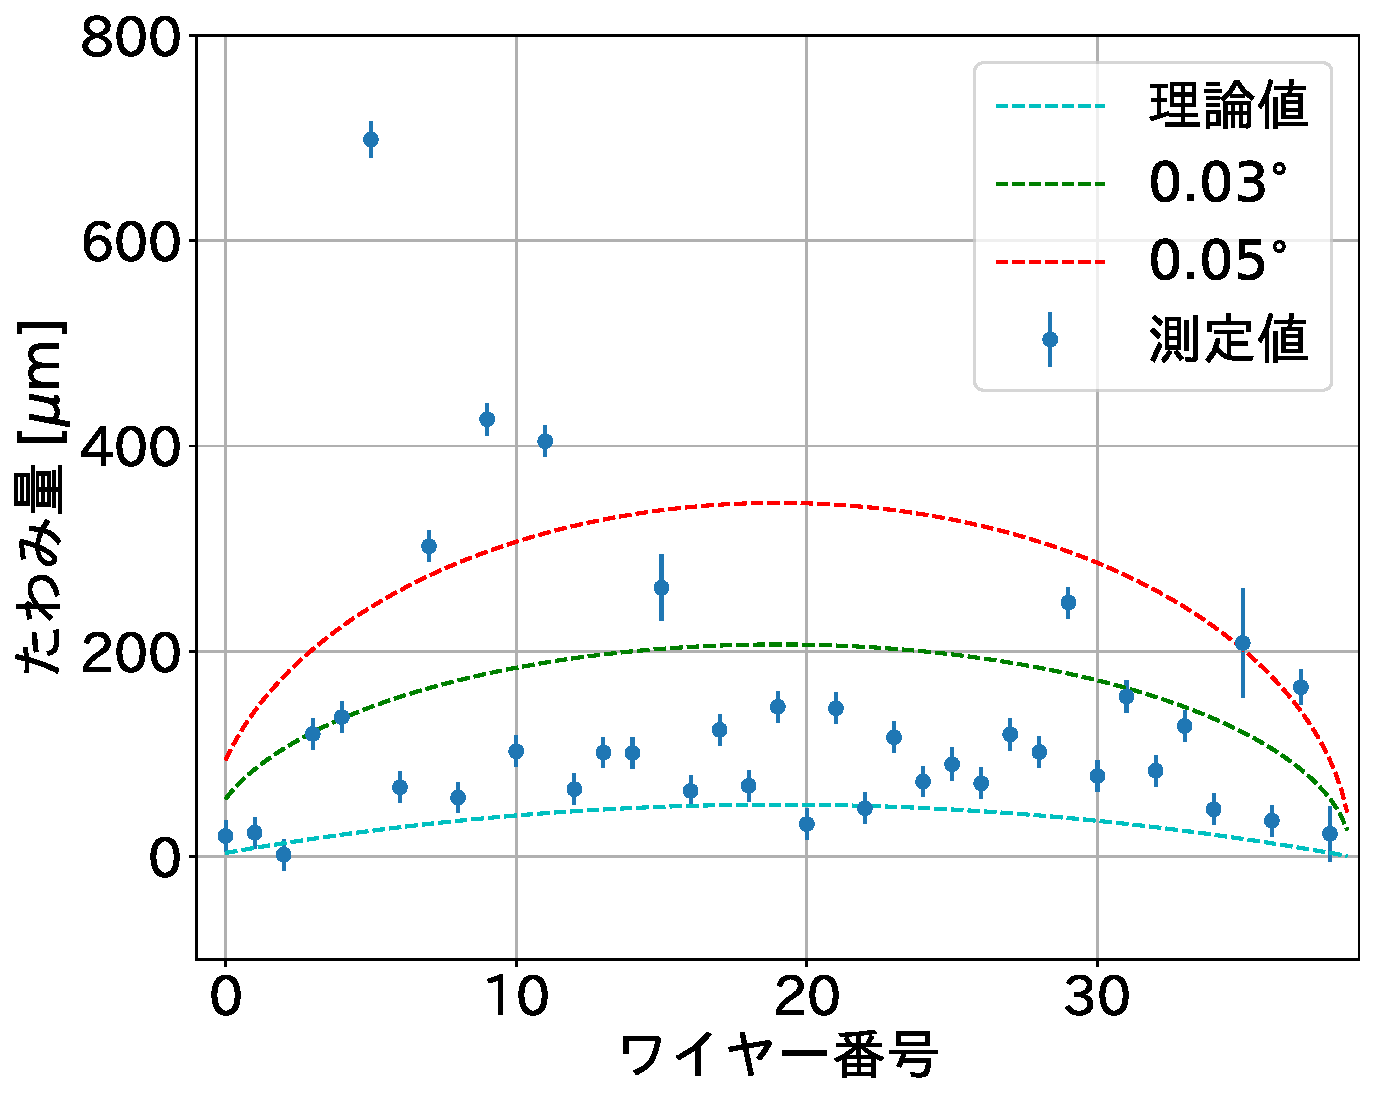
\includegraphics[width=1.0\textwidth]{wiresag_swg/swg_sag_before.pdf}
        \subcaption{}
        \label{fig:wiresag_swg_sag_result}
    \end{minipage}
    \begin{minipage}[b]{0.5\hsize}
        \centering
        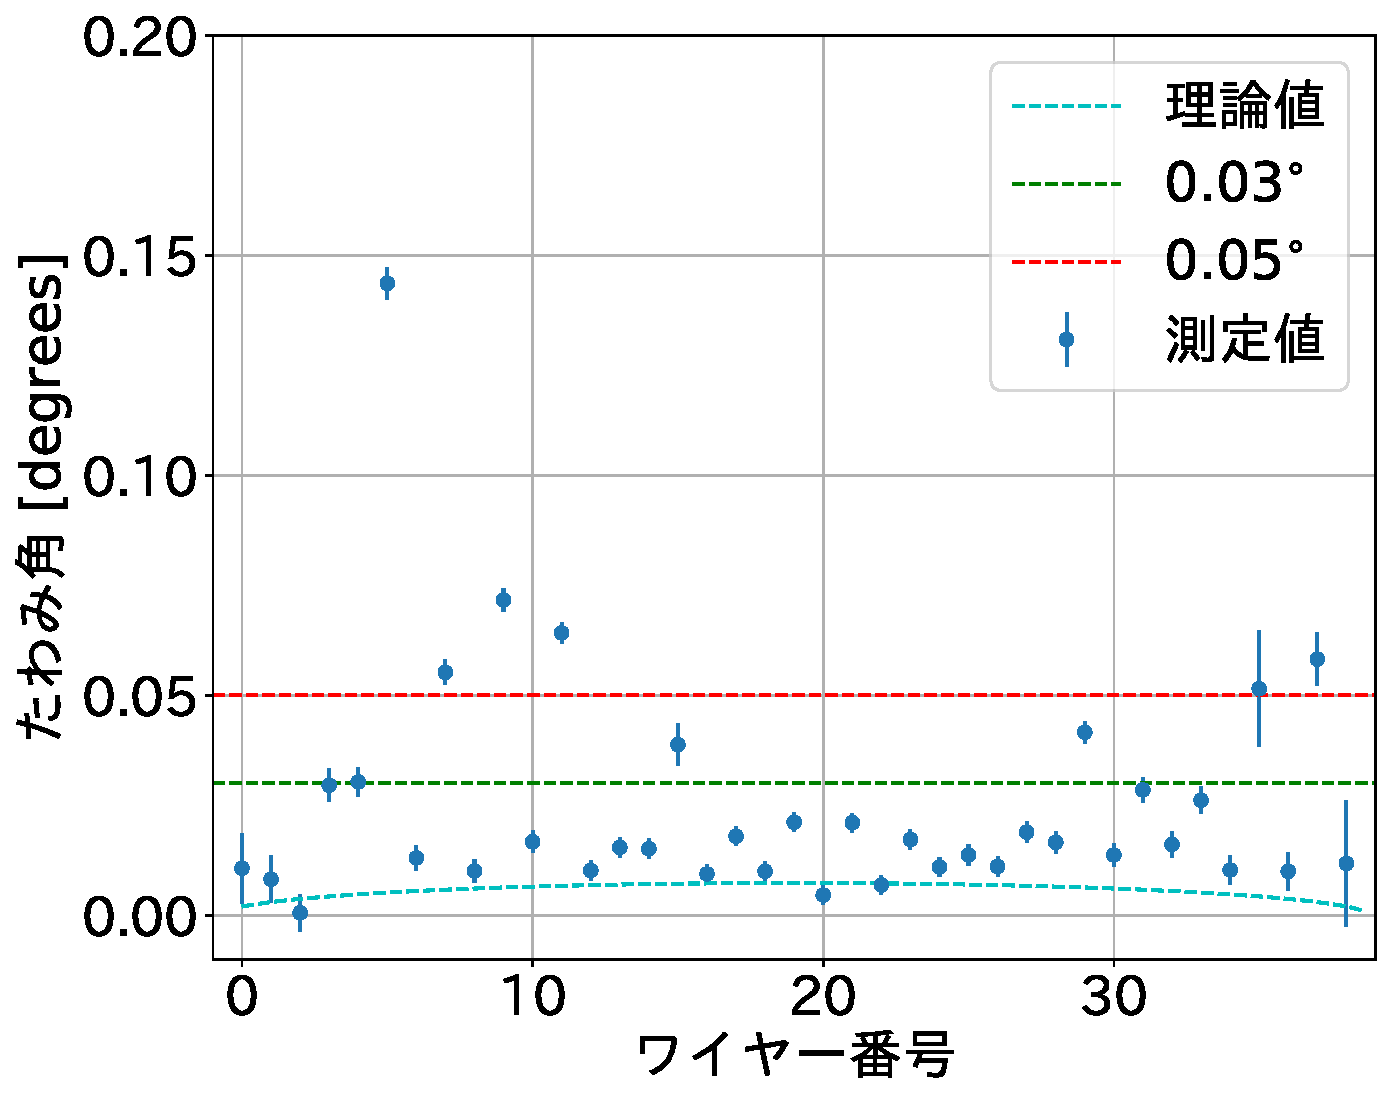
\includegraphics[width=1.0\textwidth]{wiresag_swg/swg_sag_angle_before.pdf}
        \subcaption{}
        \label{fig:wiresag_swg_sag_angle_result}
    \end{minipage}
    \caption{(\subref{fig:wiresag_swg_sag_result}) スパースワイヤーグリッドのたわみ量の評価結果。\ 
             (\subref{fig:wiresag_swg_sag_angle_result}) たわみ量を角度に変換したもの。}
    \label{fig:wiresag_swg_result}
\end{figure}
\begin{figure}[H]
    \centering
    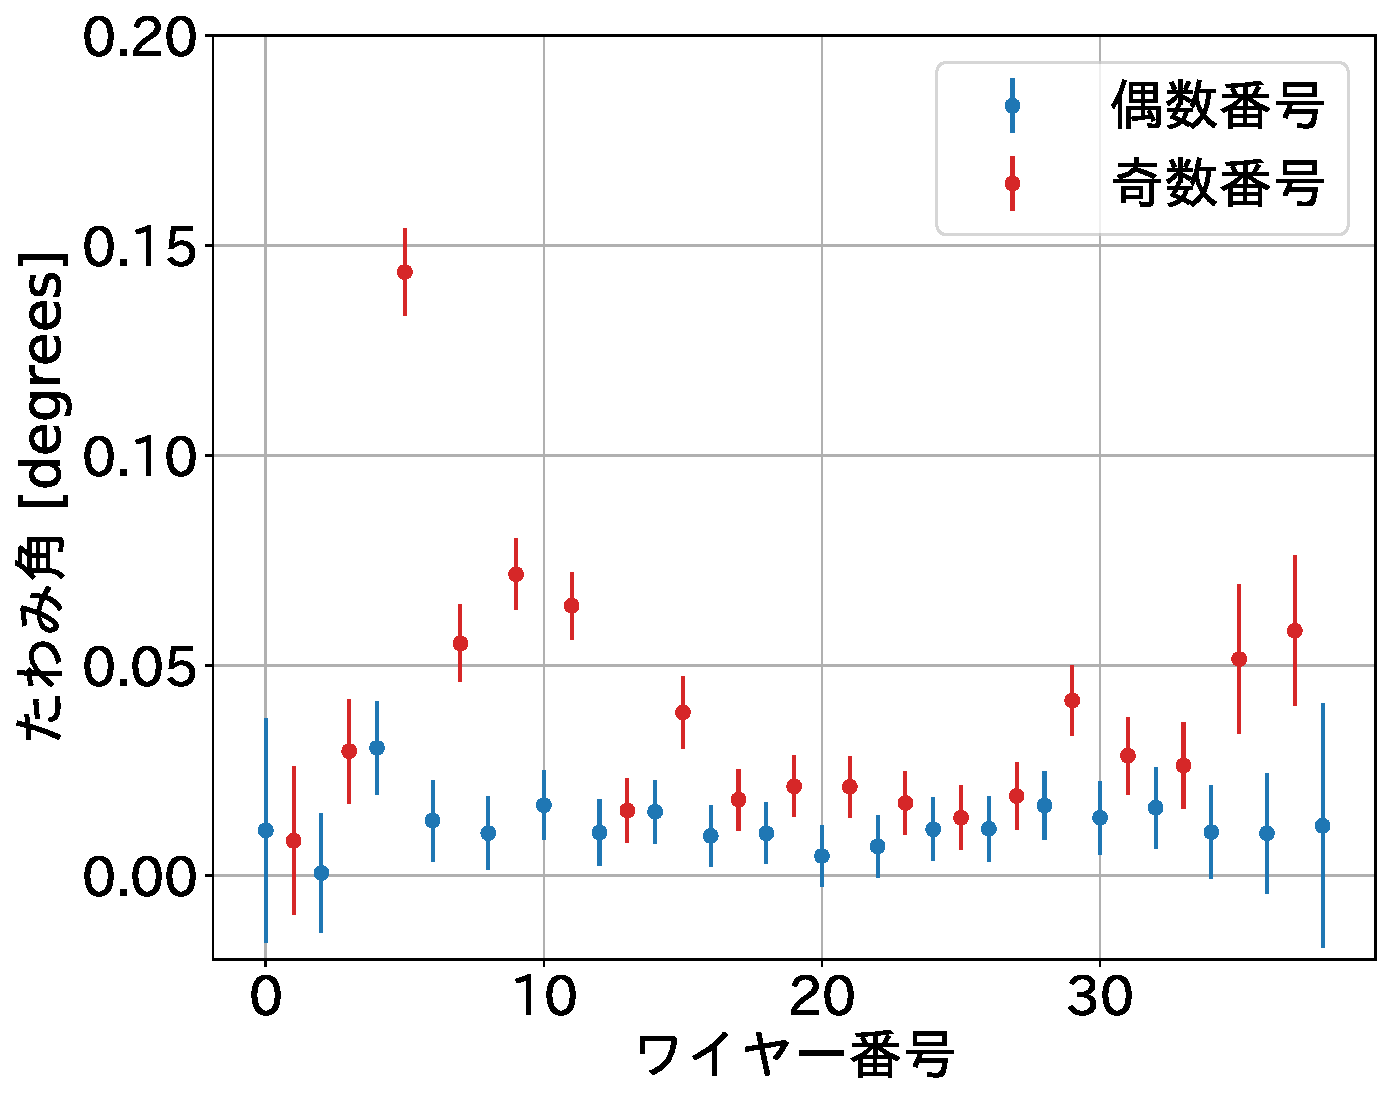
\includegraphics[width=0.7\textwidth]{wiresag_swg/swg_sag_angle_before_even_odd.pdf}
    \caption{ワイヤー番号の偶奇によるたわみ角の違い。
    全体的に奇数番号のワイヤーの方が偶数番号のワイヤーと比較してたわみ角が大きい傾向にある。}
    \label{fig:wiresag_swg_even_odd}
\end{figure}

\section{奇数番目のワイヤーを修繕後の評価結果とその考察}
奇数番目のワイヤーを外し、再度張り直すことで修繕されたスパースワイヤーグリッドのたわみ量を評価した。
修繕後のスパースワイヤーグリッドのたわみ量の評価結果を図\ref{fig:wiresag_swg_result_repair}(\subref{fig:wiresag_swg_sag_result_repair})に、
たわみ角の評価結果を図\ref{fig:wiresag_swg_result_repair}(\subref{fig:wiresag_swg_sag_angle_result_repair})に示す。
どちらの図中にも、比較のために修繕前の評価結果もあわせて示している。
得られたたわみ角の平均は$0.020\tcdegree$であり、修繕前のたわみ角の平均$0.025\tcdegree$よりも$0.005\tcdegree$改善した。
また、修繕前にたわみ角が$0.05\tcdegree$を超えるワイヤーは6本存在していたが、修繕後には2本に減少している。
これらの結果は、本装置を用いてワイヤーのたわみ量を評価することにより、品質の悪いワイヤーを張り直してたわみ量を改善可能であることを示している。

% 修繕前後での評価されたワイヤーのたわみ量の比較を図\ref{fig:wiresag_swg_result_repair_compare}に示す。
% また、たわみ角についても同様に比較した図を図\ref{fig:wiresag_swg_result_repair_angle_compare}に示す。

% したがって、これらの和をとることにより修繕後のワイヤーのたわみが与える望遠鏡の偏光角較正への影響は
% $\theta_{\mathrm{sag}}=0.030\tcdegree$であり、修繕前の$\theta_{\mathrm{sag}}=0.036\tcdegree$よりも小さくなった。

ただし、奇数番目のワイヤー修繕後に、偶数番目のワイヤーでたわみが増加してしまったものがある。そのことを示す図を、図\ref{fig:wiresag_swg_even_odd_repair_comparison}(\subref{fig:wiresag_swg_sag_odd_comparison})(\subref{fig:wiresag_swg_sag_even_comparison})に示す。
図\ref{fig:wiresag_swg_even_odd_repair_comparison}(\subref{fig:wiresag_swg_sag_odd_comparison})は奇数番目のワイヤーのたわみ量を修繕前後で比較した結果、
図\ref{fig:wiresag_swg_even_odd_repair_comparison}(\subref{fig:wiresag_swg_sag_even_comparison})は偶数番目のワイヤーのたわみ量を修繕前後で比較した結果である。
これらの図から、奇数番目は修繕によりたわみ角が小さくなっているが、偶数番目は修繕により大きくなっていることがわかる。
修繕は奇数番目のワイヤーのみを張り直すことで行われたため、スパースワイヤーグリッドのワイヤーは2回に分けて張ることにより、先に張られたワイヤーがたわんでしまうことがわかった。

今回の修繕(1回目)では、たわみ角が$0.05\tcdegree$を超えるワイヤーが6本から2本に減った。
しかし、以前としてたわみ角が$0.05\tcdegree$を超えるワイヤーが存在している。
そこで、この2本のワイヤーのみを張り直し、修繕(2回目)を行う。
これにより、その他のワイヤーのたわみ角を悪化させずに2本のみを修繕することができるか検証した。

% 2本品質の悪いワイヤーはあるものの、今回の修繕後の結果を用いて、ワイヤーのたわみに起因する望遠鏡の偏光角較正への影響を算出する。
% 修繕後のワイヤーのたわみ角の平均値は$0.020\tcdegree$(これは品質の悪い2本を入れた値であり、それらを除くと$0.015\tcdegree$)、たわみ角の誤差の平均値は$0.003\tcdegree$であった。
% 先行研究にしたがい、これらの和をありうる最大のたわみ角とすると、$\theta_{\mathrm{sag}}=0.023\tcdegree<0.03\tcdegree$といえる。
% よって、先行研究で得られた$\theta_{\mathrm{sag}}<0.05\tcdegree$よりも$\SI{40}{\%}$たわみによる偏光角較正の誤差を改善することができた。
% 明らかに品質の悪い$4,\,6$番目の以外の偶数番目のワイヤーで、修繕前後のたわみ角の変化の平均値を算出すると$0.01\tcdegree$であった。
\begin{figure}[H]
    \begin{minipage}[b]{0.5\hsize}
        \centering
        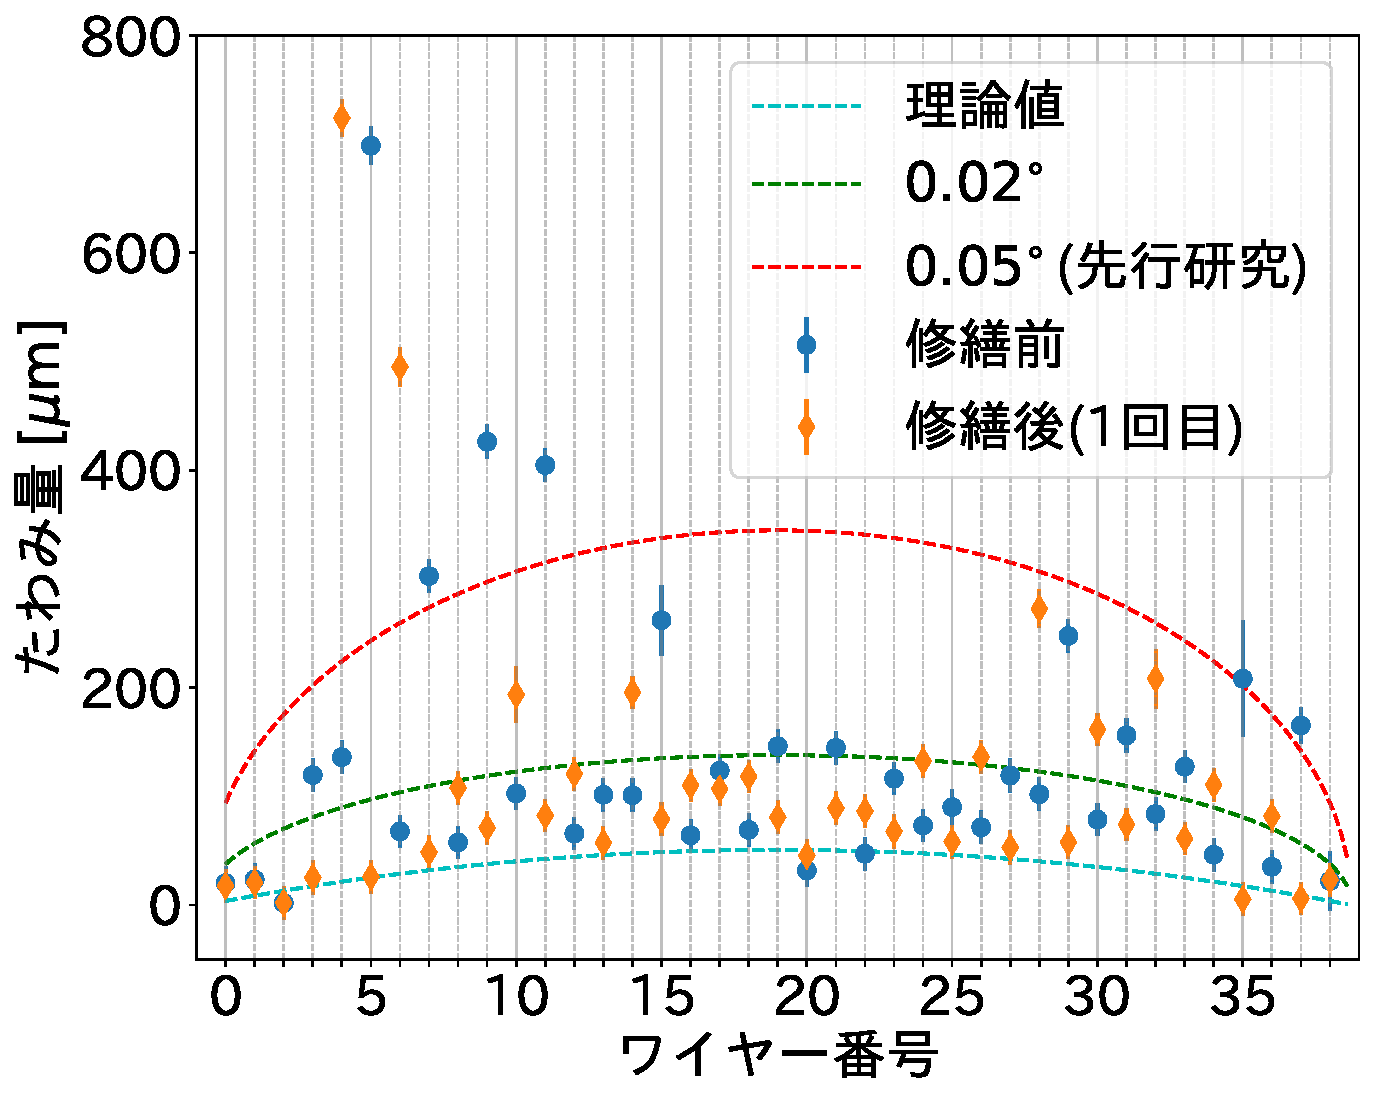
\includegraphics[width=1.0\textwidth]{wiresag_swg/swg_sag_comparison.pdf}
        \subcaption{}
        \label{fig:wiresag_swg_sag_result_repair}
    \end{minipage}
    \begin{minipage}[b]{0.5\hsize}
        \centering
        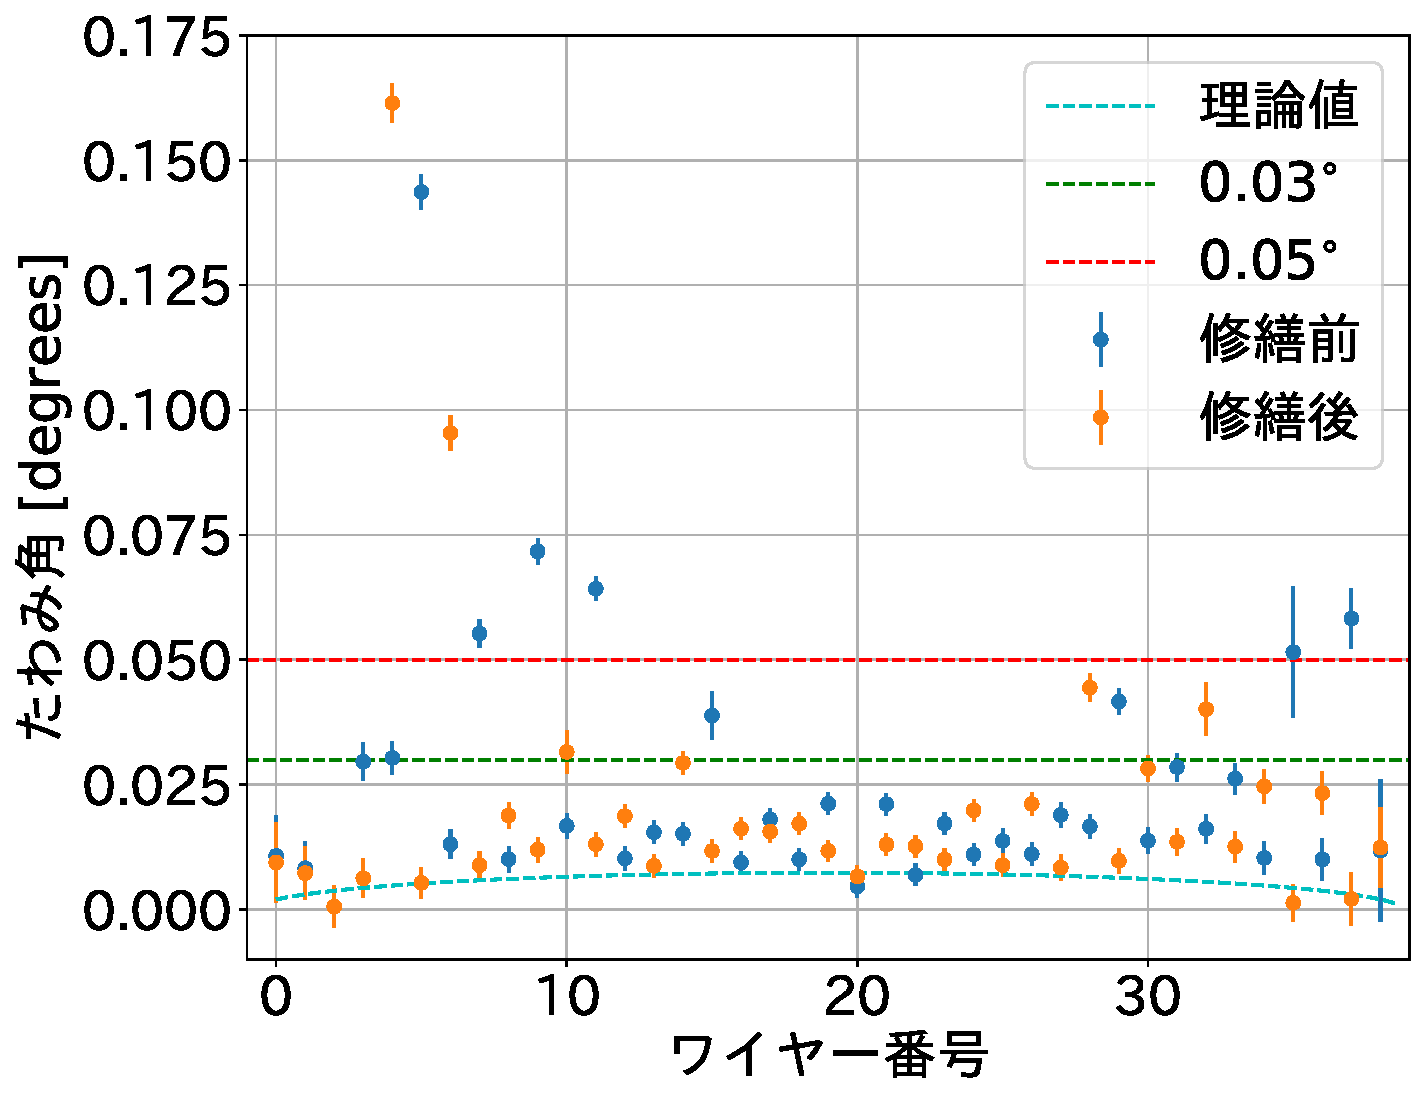
\includegraphics[width=1.0\textwidth]{wiresag_swg/swg_sag_angle_comparison.pdf}
        \subcaption{}
        \label{fig:wiresag_swg_sag_angle_result_repair}
    \end{minipage}
    \caption{作成直後のスパースワイヤーグリッドのたわみの評価結果と、奇数番目を張り直し、1回目の修繕を行った後のスパースワイヤーグリッドのたわみの評価結果の比較。
             (\subref{fig:wiresag_swg_sag_result_repair}) 修繕後のスパースワイヤーグリッドのたわみ量の評価結果。
             (\subref{fig:wiresag_swg_sag_angle_result_repair}) 修繕後のスパースワイヤーグリッドのたわみ角の評価結果。
             $0.05\tcdegree$を超えるたわみ角を有していたワイヤーが6本から2本に改善されている。}
    \label{fig:wiresag_swg_result_repair}
\end{figure}
\begin{figure}[H]
    \begin{minipage}[b]{0.5\hsize}
        \centering
        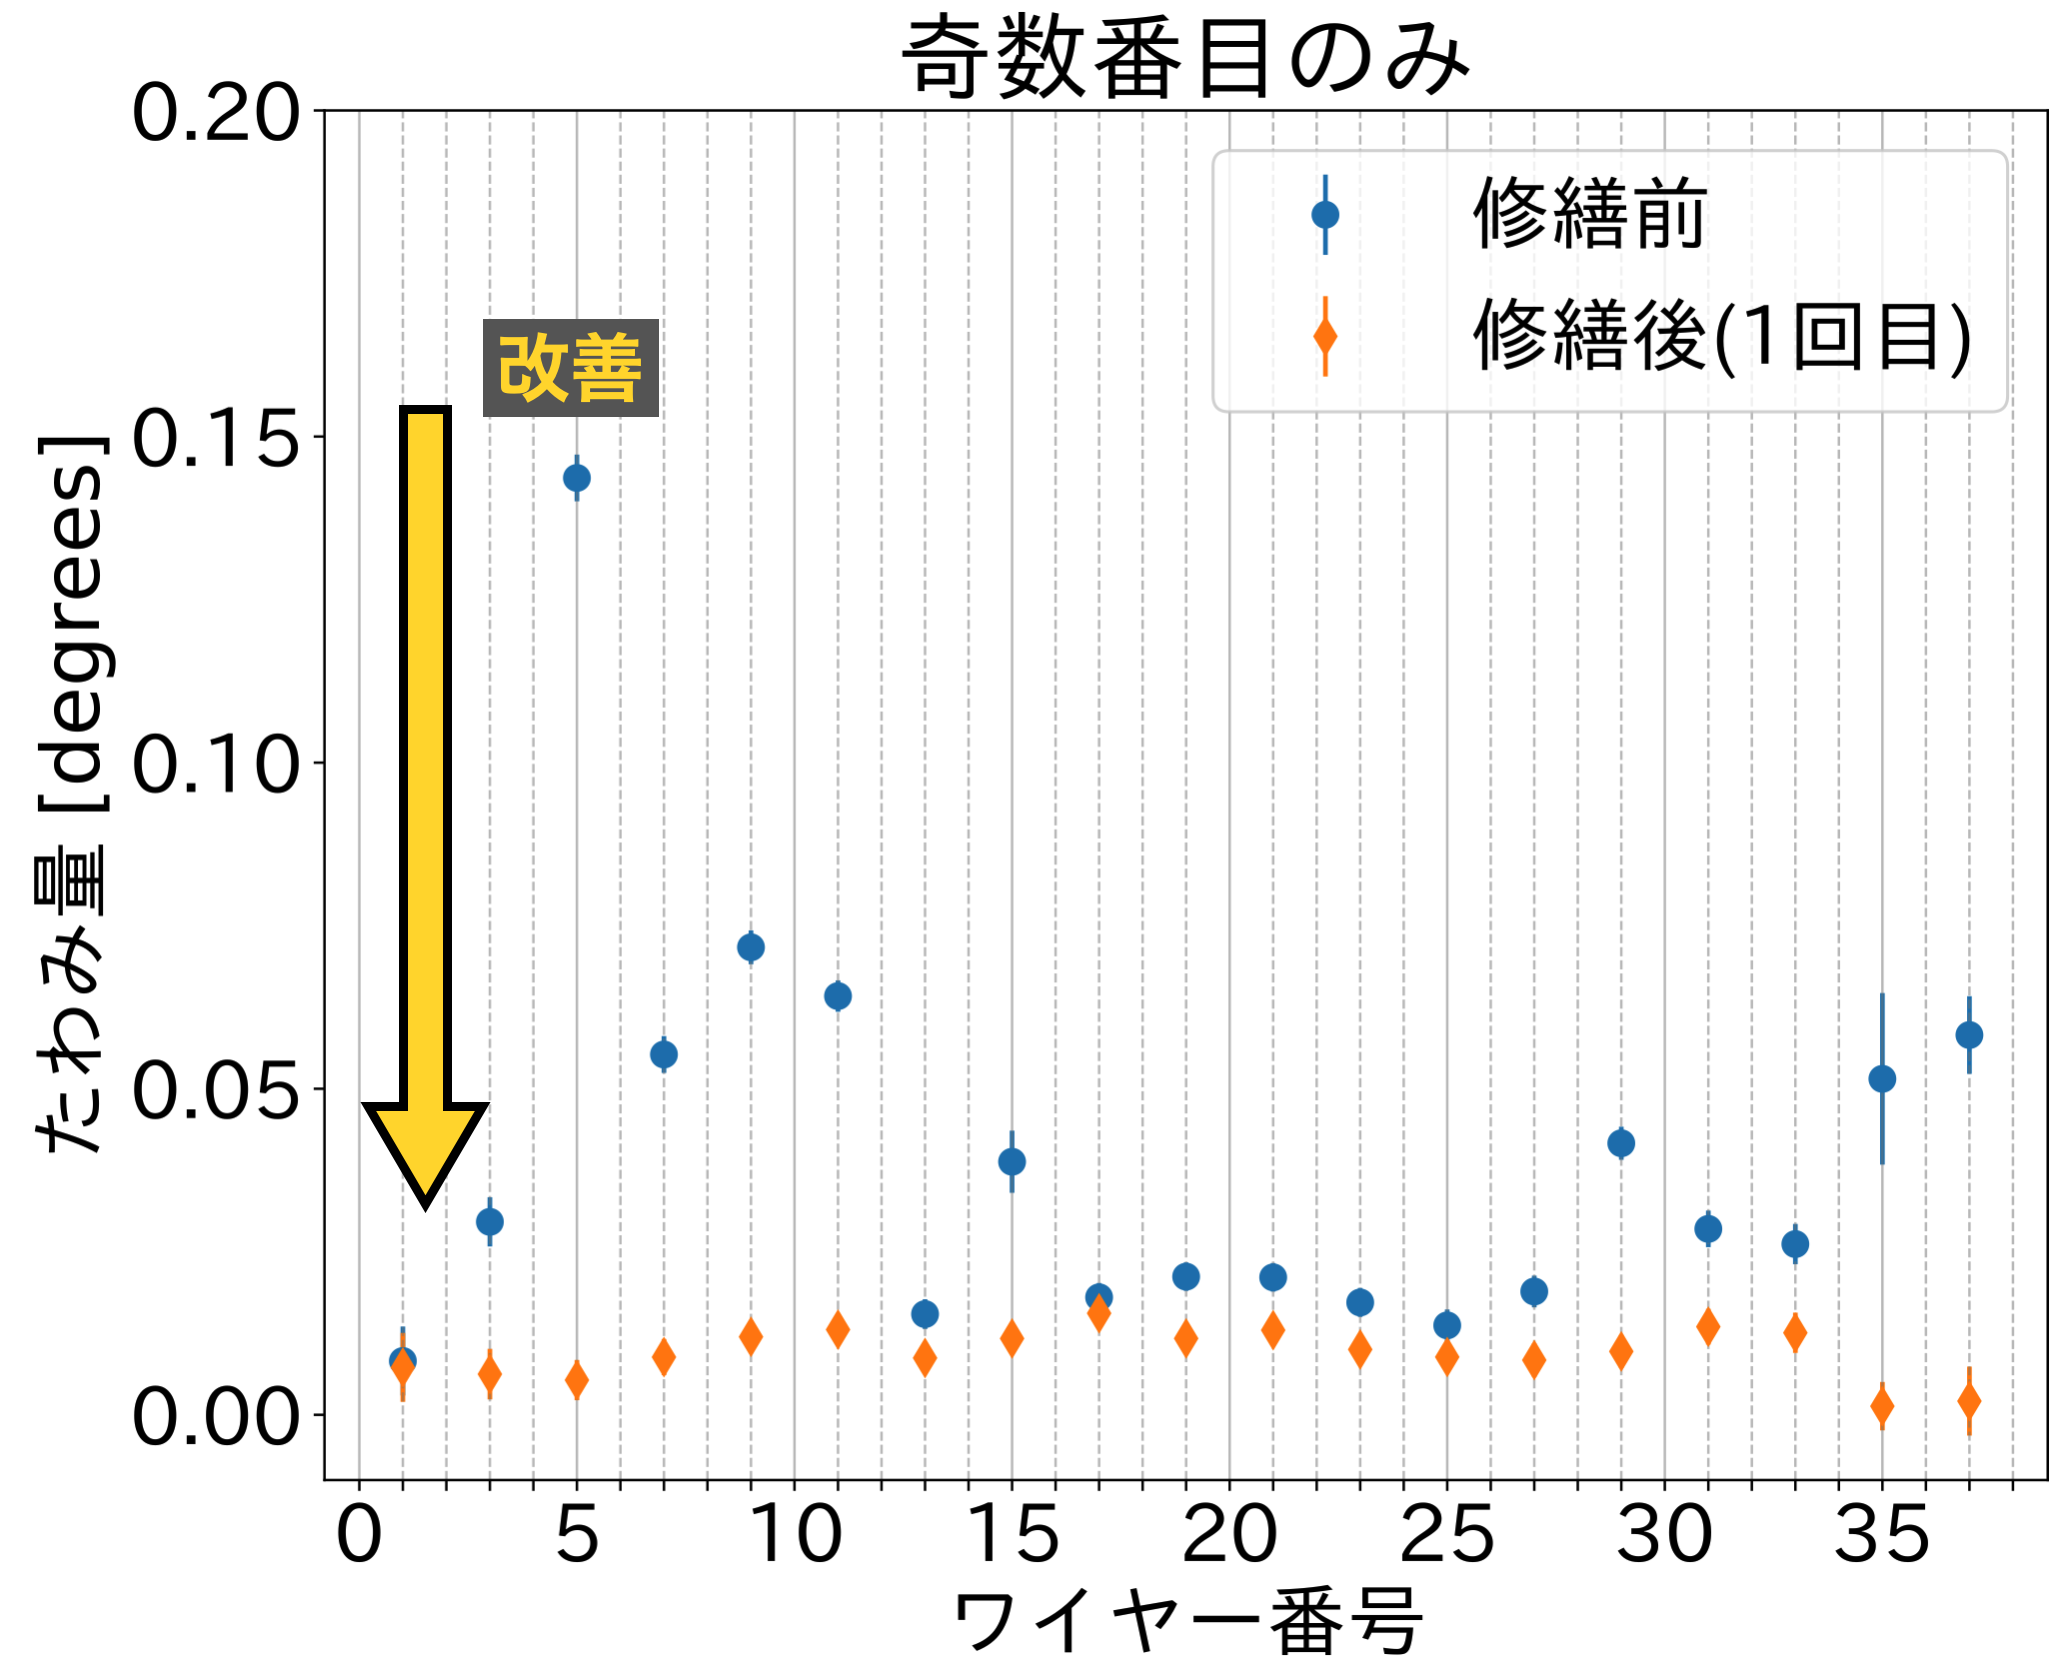
\includegraphics[width=1.0\textwidth]{wiresag_swg/swg_sag_angle_odd_comparison.png}
        \subcaption{}
        \label{fig:wiresag_swg_sag_odd_comparison}
    \end{minipage}
    \begin{minipage}[b]{0.5\hsize}
        \centering
        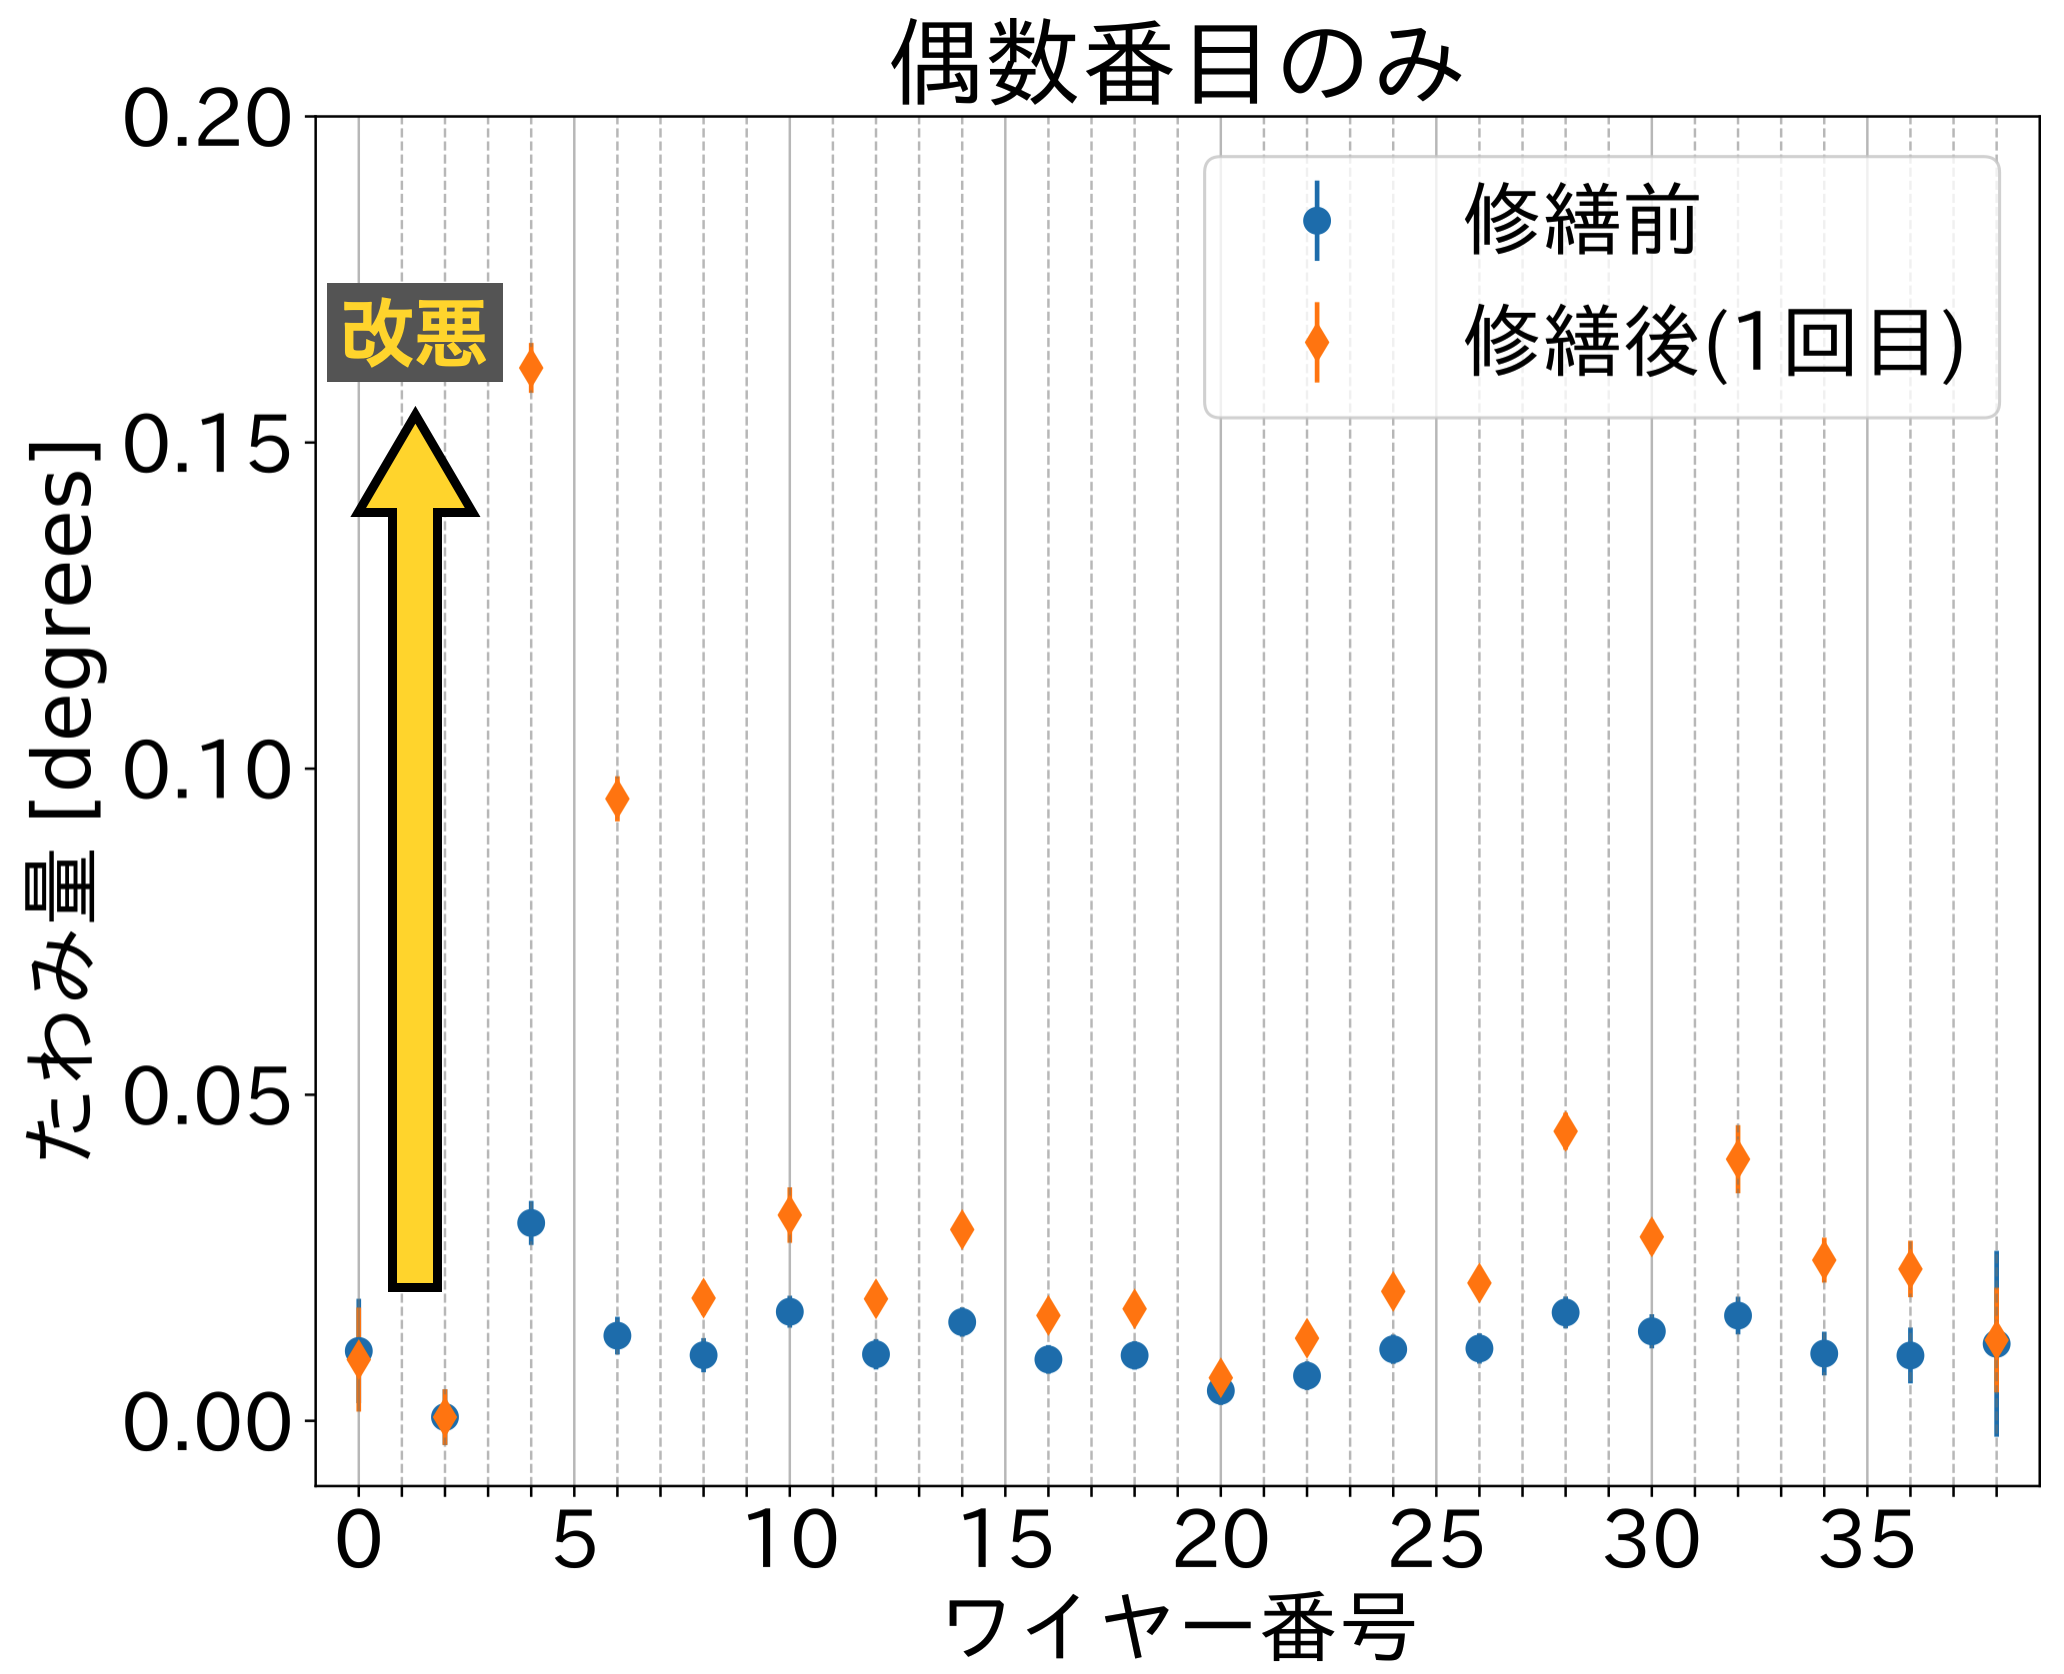
\includegraphics[width=1.0\textwidth]{wiresag_swg/swg_sag_angle_even_comparison.png}
        \subcaption{}
        \label{fig:wiresag_swg_sag_even_comparison}
    \end{minipage}
    \caption{(\subref{fig:wiresag_swg_sag_odd_comparison}) 奇数番目のワイヤーのたわみ角の修繕前後での比較。修繕後の方が小さくなっており、改善している。\ 
             (\subref{fig:wiresag_swg_sag_even_comparison}) 偶数番目のワイヤーのたわみ角の修繕前後での比較。
             修繕後の方が大きくなっており、修繕時に張り直されなかったワイヤーはたわみ角が大きくなることを示唆する。
             }
    \label{fig:wiresag_swg_even_odd_repair_comparison}
\end{figure}

\section{たわみ角が$0.05\tcdegree$以上であるワイヤーを修繕後の評価結果とその考察}
前節にてたわみ角が$0.05\tcdegree$以上であると評価された2本のワイヤーのみを張り直し、2回目の修繕を行ったスパースワイヤーグリッドのたわみ量を評価した。
修繕後のたわみ量の評価結果を図\ref{fig:wiresag_swg_result_repair2}(\subref{fig:wiresag_swg_sag_result_repair2})に、
たわみ角の評価結果を図\ref{fig:wiresag_swg_result_repair2}(\subref{fig:wiresag_swg_sag_angle_result_repair2})に示す。
どちらの図にも、前節にて行った奇数番目のワイヤーを修繕後(1回目)の評価結果を比較のために合わせて示している。
貼り直された2本はたわみ角が理論値程度まで改善しており、その他のワイヤーのたわみ角も悪化していないことがわかる。
2回目の修繕後のたわみ角の平均値は$0.012\tcdegree$であり、1回目の修繕後のたわみ角の平均値$0.020\tcdegree$から$0.009\tcdegree$改善した。
以上の結果から、本装置を用いてたわみ角の大きい($<0.05\tcdegree$)ワイヤーの選別し、張り直すことを繰り返すことで、
スパースワイヤーグリッドの平均たわみ角を$0.01\tcdegree$程度まで改善することが可能であることが示された。

今回の修繕(2回目)の結果を用いて、ワイヤーのたわみに起因する望遠鏡の偏光角較正への影響を算出する。
修繕後のワイヤーのたわみ角の平均値は$0.012\tcdegree$、たわみ角の誤差の平均値は$0.003\tcdegree$であった。
先行研究\cite{swg:murata}\cite{swg:iijima}にしたがい、これらの和をありうる最大のたわみ角とすると、$\theta_{\mathrm{sag}}=0.015\tcdegree<0.02\tcdegree$といえる。
よって、先行研究で得られた$\theta_{\mathrm{sag}}<0.05\tcdegree$よりも$\SI{60}{\%}$たわみによる偏光角較正の誤差を改善することができた。


\begin{figure}[H]
    \begin{minipage}[b]{0.5\hsize}
        \centering
        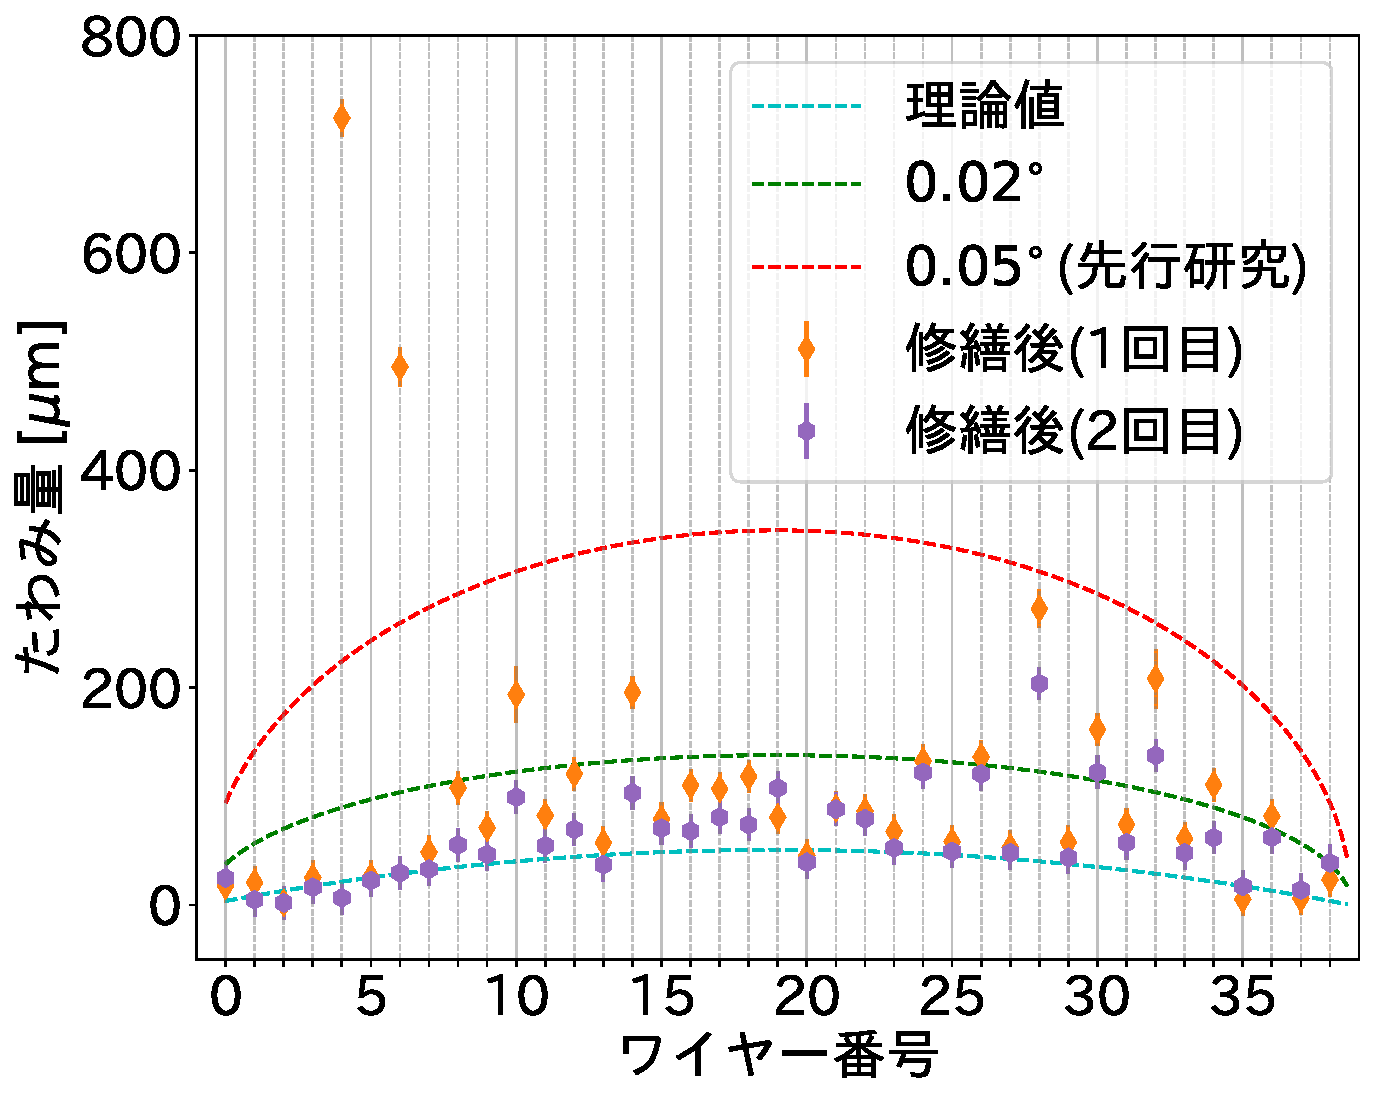
\includegraphics[width=1.0\textwidth]{wiresag_swg/swg_sag_comparison2.pdf}
        \subcaption{}
        \label{fig:wiresag_swg_sag_result_repair2}
    \end{minipage}
    \begin{minipage}[b]{0.5\hsize}
        \centering
        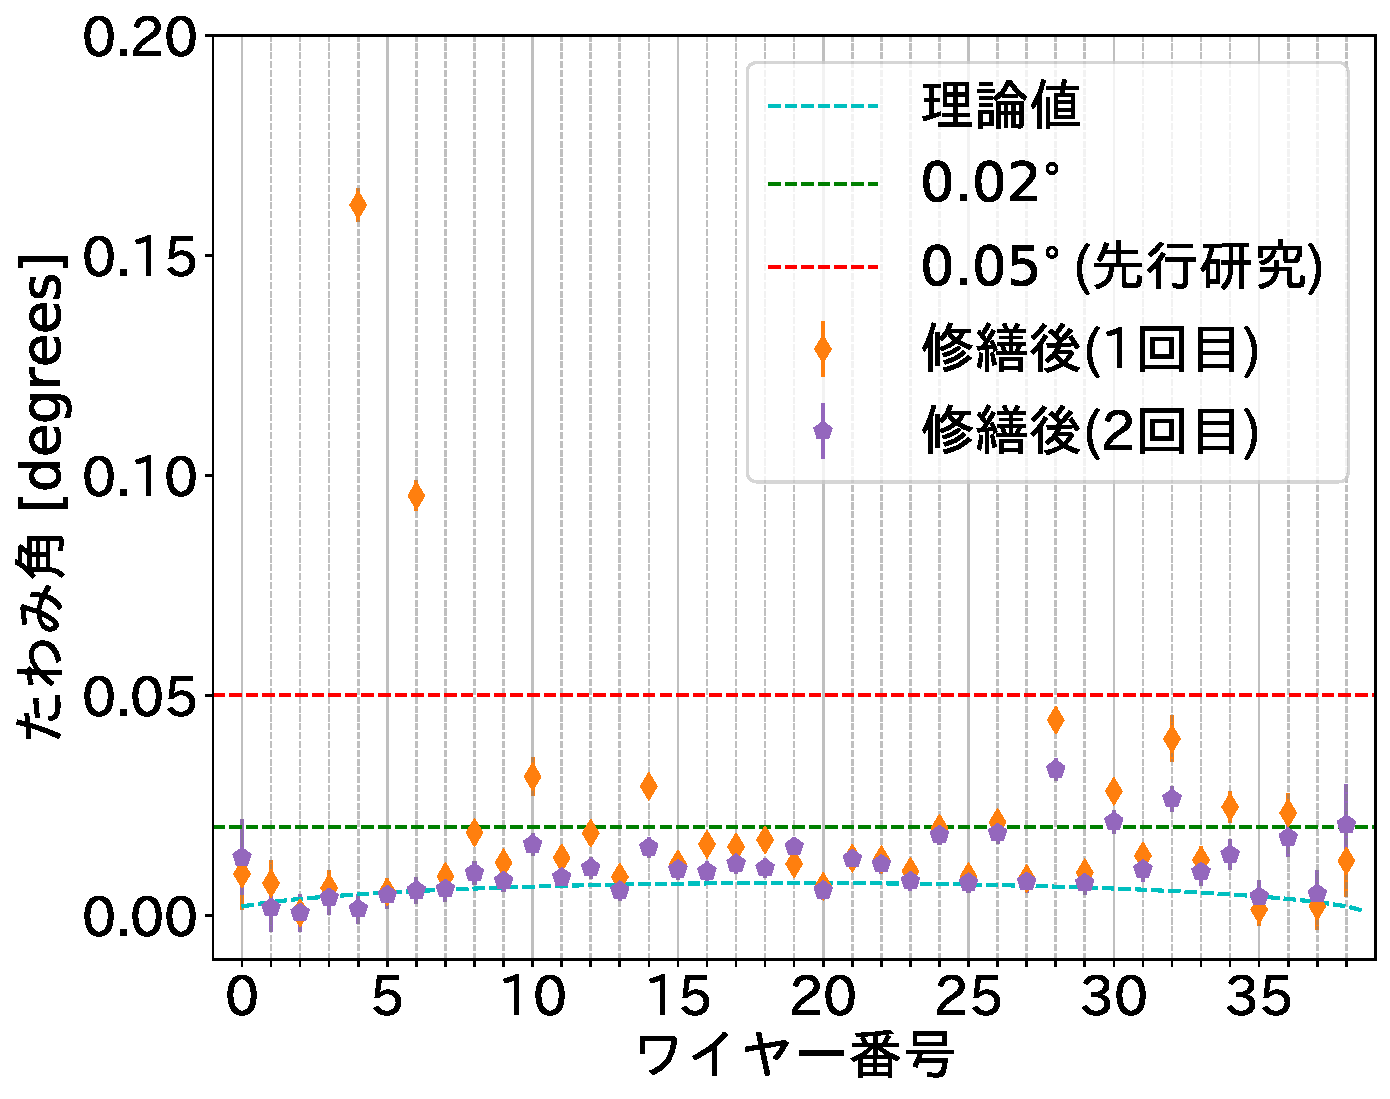
\includegraphics[width=1.0\textwidth]{wiresag_swg/swg_sag_angle_comparison2.pdf}
        \subcaption{}
        \label{fig:wiresag_swg_sag_angle_result_repair2}
    \end{minipage}
    \caption{1回目の修繕後のスパースワイヤーグリッドのたわみの評価結果と、$0.05\tcdegree$を超えるたわみ角を有していた2本のワイヤーを張り直し、2回目の修繕を行ったスパースワイヤーグリッドのたわみの評価結果の比較。
             (\subref{fig:wiresag_swg_sag_result_repair2}) 修繕後のスパースワイヤーグリッドのたわみ量の評価結果。
             (\subref{fig:wiresag_swg_sag_angle_result_repair2}) 修繕後のスパースワイヤーグリッドのたわみ角の評価結果。
             $0.05\tcdegree$を超えるたわみ角を有していたワイヤーが2本から0本に改善されている。}
    \label{fig:wiresag_swg_result_repair2}
\end{figure}

\section{まとめと今後の展望}
本章では、開発したワイヤーのたわみ量の自動評価装置を用いて、望遠鏡の偏光角較正に使用されるスパースワイヤーグリッドのたわみ量を評価した。
最初に評価されたワイヤーのたわみ角の平均値は$0.025\tcdegree$であったが、たわみ角が大きいワイヤーを張り直すことでたわみ角の平均値は$0.020\tcdegree$に改善された。
また、この修繕前にはたわみ角が$0.05\tcdegree$を超えるワイヤーが6本存在していたが、修繕によって2本に減らすことができた。
以上から、本装置を用いてたわみ角が大きいワイヤーを選別し、ワイヤーを張り直すことでたわみ角を改善可能であることが示された。
修繕後のスパースワイヤーグリッドにおいて、たわみ角が偏光角較正へ与える影響を算出したところ、$\theta_{\mathrm{sag}}<0.030\tcdegree$であった。
この評価値は先行研究にて与えられる$\theta_{\mathrm{sag}}<0.05\tcdegree$から$\SI{40}{\%}$改善された値である。
また、スパースワイヤーグリッドのワイヤーを偶数番目、奇数番目の2回に分けて張ることにより、
先に張られたワイヤーがたわんでしまう可能性があることがわかった。

今後の展望として、まず今回評価したスパースワイヤーグリッドに関して、品質の悪い2本のワイヤーをだけ張り直す。
これによって張り直されたワイヤーのたわみ角が張り直す前の平均値$0.025\tcdegree$程度に抑えられれば、
張り直した後のたわみ角の平均値は$0.016\tcdegree$程度に改善できる。
各たわみ角の誤差が$0.003\tcdegree$から変わらなければ、ワイヤーのたわみによる偏光角較正への影響$\theta_{\mathrm{sag}}$は$\theta_{\mathrm{sag}}<0.02\tcdegree$に抑えられる。
また、本研究により、ワイヤーを張る手順に伴うリングの歪みがワイヤーのたわみの要因であることがつきとめられた。
今後新たにスパースワイヤーグリッドにワイヤーを張る際には、すべてのワイヤーを同時に張るように張り方を改善することを提案する。
% たわみ量をさらに抑えるためにはスパースワイヤーグリッドのワイヤーを張る工程を改善することが重要である。
% まずはワイヤーをすべて同時に張ることで、ワイヤーのたわみ量を均一に抑えることができるか調べる必要がある。

% これによりワイヤーがスパースワイヤーグリッドのリングを歪めているかどうかを検証できる。
% また、張力によりワイヤーがスパースワイヤーグリッドのリングを歪めているのであれば、リングの構造を歪みに対して強力なものに変更するか、
% ワイヤーにかける張力を弱めることでさらなるたわみ量の改善が見込まれる。
\end{document}